\documentclass[11pt]{article}
\usepackage[spanish]{babel}
\usepackage[utf8]{inputenc}
\usepackage{geometry}
\usepackage{booktabs}  
\usepackage{subfig,graphicx} 
\usepackage{listings}
\usepackage{amsmath,amsthm,amssymb}
\usepackage{float}

\lstset{%
backgroundcolor=\color{cyan!10},
basicstyle=\ttfamily,
numbers=left,numberstyle=\scriptsize
}

\setlength{\parskip}{\baselineskip}%
\setlength{\parindent}{0pt}%

%\usepackage[wby]{callouts}
\usepackage{url}
\usepackage{hyperref}

\title{Memoria del Proyecto Final}
\author{Álvaro Beltrán Camacho \\ Yábir García Benchakhtir}
\begin{document}

\maketitle

\begin{figure}[h]

\includegraphics[scale=0.3]{UGR}
\centering
\end{figure}

\newpage

\renewcommand*\contentsname{Índice}
\tableofcontents

\newpage

\section{Definición del problema a resolver y enfoque elegido}

Para nuestro proyecto nos hemos decantado por trabajar con el conjunto de datos
\textit{Adult Census Income} recogido por Ronny Kohavi y Berry Becker \cite{dataset}. 

Se nos presenta un conjunto muestras para las que se han recogido distintos
parámetros que pueden afectar a la cantidad de dinero que se ingresa. Las
variables, las cuales se analizarán posteriormente, abarcan desde la edad
hasta el país de origen y el problema consiste en determinar cuando una muestra
va superar las 50000 unidades monetarias de ingresos y cuando se va a mantener
por debajo.

Estamos ante un problema de aprendizaje supervisado en el ámbito de la
clasificación binaria. En nuestro caso los elementos que intervienen en el
aprendizaje son 

\begin{itemize}
    \item $X$: Conjunto de datos relativos a una persona que pueden tener
    repercusión en el dinero que gane. Se trata de un vector que mezcla
    variables categóricas con variables reales.
    \item $y$: Es un valor en el conjunto $\{0,1\}$ que nos indica si los
    ingresos superan las 50000 unidades monetarias o no.
    \item $f$: Función que nos relaciona el conjunto $X$ con $y$ de manera que a
    cada muestra le asigna su categoria de ingresos.
\end{itemize}

En este problema es dicha función $f$ la que queremos aproximar. Para ello vamos
a basar nuestro estudio en aplicar el conocimiento adquirido durante la
asignatura utilizando métodos lineales y no lineales.

\section{Obtención de los datos}

Para la obtención de los datos hemos utilizado el repositorio público de
\textit{UCI}, más concretamente la url
\href{https://archive.ics.uci.edu/ml/machine-learning-databases/adult/}{https://archive.ics.uci.edu/ml/machine-learning-databases/adult/}.
Podemos apreciar como hay distintos archivos entre los que se encuentran los
datos y una descripción. 

Los datos aparecen separados en dos archivos distintos, uno para training y otro
para test. Descargamos ambos ficheros (\textit{adult.data}, \textit{adult.test})
y en nuestro trabajo hemos decidido combinarlos para realizar una separación
propia.

El motivo de esta elección es que como se verá a continuación hay un alto número
de muestras del total disponible a las que le falta el valor de alguna columna.
Como en general son unas columnas concretas en las que las muestras no estan
provistas del valor, se ha seguido el criterio expuesto en el guión de asignar
un valor aleatorio en función de una distribución multinomial. Es por esto que
hemos creido correcto que era mejor juntar los datos, aproximar los valores que
faltaban y crear conjuntos de test y training basados en una poporción 80-20
(80\% de los datos para training y 20\% para test).

\section{Argumentos a favor de la elección de los modelos.}

En cuanto a los modelos lineales elegidos nos hemos decantado por Regresión
Logística y Perceptron, debido a que son dos modelos que hemos estudiado en
clase para ejemplos de clasificación binaria, como es nuestro caso.  

Además parece interesante probar con el Perceptron puesto que también vamos a
usar el perceptron multicapa (MLP). Y puesto que Regresión Logística ha dado tan
buenos resultados en las prácticas de esta asignatura y suele funcionar muy bien
en clasificación parece indispensable probar este modelo.

De los modelos no lineales propuestos hemos elegido Perceptron Multicapa, Random
Forest y SVD.

Vamos a usar Ramdom Forest por que suele ser bueno para problemas de clasificación
y poco sensible a cambios en el conjunto de train (vamos a usar
validación cruzada).

Perceptron Multicapa es un modelo que nos permite aprender funciones no lineales
utilizando la técnica de \textit{backpropagation}. Este tipo de algoritmos son
interesantes ya que nos permiten aprender relaciones entre las variables y cual
es la mejor manera con la que relacionarlas con nuestra función de salida. Es
por esto que esta técnica tiene gran interés y por lo que nosotros hemos
decidido usarala.

SVC. En nuestro caso nos hemos decantado por utilizar también un algoritmo de tipo
Suport Vector Machine preparado para hacer clasificación. Hemos visto que es una 
técnica muy potente que puede darnos muy buenos resultados cuando tenemos un alto 
número de características. Este a priori, no es nuestro caso pero cuando, como a 
continuación veremos, recodifiquemos las variables observaremos que el número 
de variables crecerá y esta técninca nos puede proporcionar resultados de interés.

\section{Exploración y preprocesado de los datos}

En primer lugar vamos a analizar el típo de variables con los que contamos. Este
análisis lo recogemos en la siguiente tabla

\begin{table}[h!]
    \centering
    \begin{tabular}{|c|c|c|}
    \hline
    Variable & Tipo de variable & Número de categorías\\ \hline
    age & continua & - \\ \hline
    workclass & categórica & 8 \\ \hline
    fnlwgt & continua & - \\ \hline
    education & categórica & 16 \\ \hline
    education-num & continua & - \\ \hline
    marital-status & categórica & 7 \\ \hline
    occupation & categórica & 14 \\ \hline
    relationship & categórica & 6 \\ \hline
    race & categórica & 5 \\ \hline
    sex & categórica & 2 \\ \hline
    capital-gain & continua & - \\ \hline
    capital-loss & continua & - \\ \hline
    hours-per-week & continua & - \\ \hline
    native-country & categórica & 41 \\ \hline
\end{tabular}
\caption{Variables estudiadas en las muestras, su tipo y la cantidad de categorías si procede.}
\end{table}

Respecto al total del conjunto de datos nos encontramos que disponemos de
48843 muestras contando las que tenemos en los ficheros \textit{adult.data}
y \text{adult.test}. 

De estas 48843 una es una irregularidad en el archivo \textit{adult.test} que contiene 
una línea no válida.

Los datos contienen 14 columnas que se corresponden a 13 características mas 
la etiqueta que se predice. De entre las muestras las características que mas datos
perdidos tienen son 

\begin{enumerate}
    \item occupation con 2810 valoers perdidos
    \item workclass con 2800 valores perdidos 
    \item native-country con 858 valores perdidos 
\end{enumerate}

el resto de características solo tienen un valor perdido que se corresponde 
con la línea erronea en el archivo de \textit{adult.test}.

En lo que respecta al número de clases aproximadamente un $75\%$ se corresponden 
con la etiqueta $<=50K$ y un $25\%$ con la etiqueta $>50K$ (etiquetas que hemos
codificado como $0$ y $1$ respectivamente). En el siguiente gráfico se puede apreciar 
dicha diferencia en el número de muestras de cada clase 

\begin{figure}[h!]
    \centering
    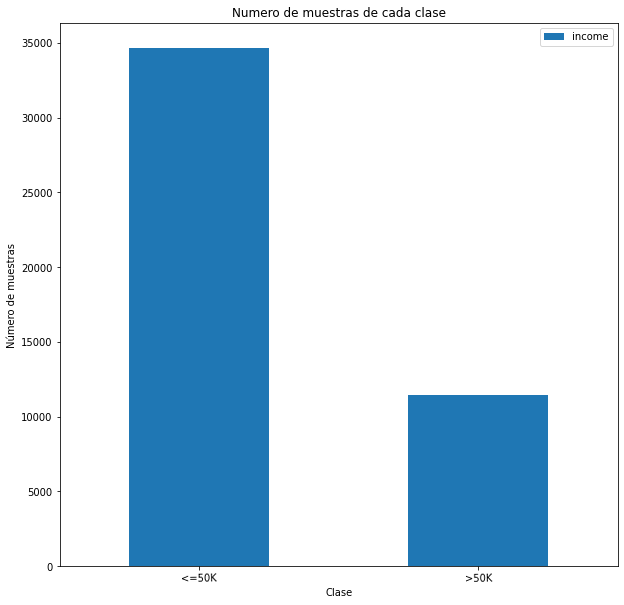
\includegraphics[width=0.7\textwidth]{images/proportion}
    \caption{Proporcion de muestras en cada clase}
\end{figure}


\subsection{Codificación de las variables}

Tenemos un conjunto de variables en las que se combinan tipos continuos y
categóricos por lo que nos va a resultar necesario convertir los datos
categóricos a valores reales. Para ello hemos optado por realizar para cada
variable de tipo categórico un vector de ceros y unos que representa con un uno
la pertenencia a una categoría concreta. Por ejemeplo en el caso de la variable
\textit{sex} que cuenta con dos categorías, $(1,0)$ representaría la pertenencia
al sexo femenino y $(0,1)$ al sexo masculino. En esta codificación de los datos
no es posible obtener un vector con más de un uno ya que en nuestros datos no se
pertenece a dos categorías de manera simultanea.

En nuestro caso nos hemos decantado por utilizar el método de pandas
\textit{get\_dummies}, que nos proporciona este comportamiento incluyendo la
codificación como variables en nuestro \textit{dataframe} de trabajo.

\subsection{Valoración del interes de las variables y selección de un subconjunto}

En principio, tras leer la descripción de los atributos estudiados. Solo vemos
dos variables que no aportan información al problema. La primera es
\textit{Education-num} que es una representación numérica del atributo education, no
aporta nada pues hemos tomado la decisión de dividir cada variable categórica en
una serie de variables donde asignamos 1 si es de un determinado tipo del
dominio de la variable o 0 si no es de ese tipo. La segunda variable es "fnlwgt"
que determina el número de personas representadas con esa instancia, entendemos
que esa variable no aporta información de fuera de la muestra y por lo tanto no
es interesante.

\subsection{Normalización de las variables}

Los rangos en los que se mueven las variables son muy dispares y normalmente con
valores muy distantes por lo que hemos visto conveniente realizar una
normalización de las variables continuas. Para ello hemos aplicado
\textit{StandardScaler} de sklearn de manera que transforma la variables
dejandolas con medio 0 y varianza 1. De esta forma  todas las variables se
encuentran centradas entorno al mismo valor y en un rango similar. 

Esto es un paso muy importante ya que afecta directamente al funcionamiento 
de los algoritmos que se van a desarrollar.

\subsection{Valores perdidos}

En cuanto a los valores perdidos hemos seguido las directrices propuestas en el
enunciado, hemos eliminado las instancias cuyos valores perdidos superaran el
10$\%$ (2 atributos con valores perdidos). Una vez eliminadas estas instancias
hemos rellenado los valores perdidos restantes con la multinomial asignando a
cada posible valor del domino del atributo una probabilidad dependiendo de la
cantidad de veces que aparecen en las instancias. Para ello, hemos usado la
función choice de la libreria random, determinando el dominio y las
probabilidades con las que aparecen cada objeto del dominio.

\subsection{Pipeline pre-entrenamiento}

De cara a entrenar nuestros modelos nos hemos decantado por se utilice la
siguiente lista ordenada de pasos en cada entrenamiento que recoge algunos de
los criterios antes comentados:

\begin{enumerate}
    \item \textit{VarianceThreshold} con un valor por defecto de 0.01
    \item \textit{StandardScaler}
    \item \textit{PolynomialFeatures} con un valor por defecto de 1
    \item \textit{LassoCV} técnica de selección de características basada en \textit{Lasso}
\end{enumerate}

El valor que hemos seleccionado para \textit{VarianceThreshold} ha sido de 0.01
basado en diferentes pruebas que hemos realizado donde, valores más altos de
este parámetro eliminaban gran cantidad de variables. Este hecho se produce por 
la introducción de las variables dummies mencionadas con anterioridad y es por esto
que finalmente nos hemos decantado por esta elección.

Respecto a la introducción de características polinómicas en las variables
introducimos un valor por defecto de 1 de manera que esta transformación no
tiene efecto en los modelos. En el caso de los modelos lineales este tipo de
transformaciones si es importante y es por esto que cuando entrenamos los modelos 
lineales propuestos estudiamos valores para este paso. 

Finalmente hemos decidido utilizar la técnica de selección de variables basada
en Lasso ya que nos permite seleccionar variables en función de la importancia
que el factor de regularización $l1$ asigna y lo hemos considerado importante ya
que con anterioridad se introducen características polinómicas. Cuando
introducimos las características polinómicas crecen sustancialmente  el número
de características y creemos que esto puede provocar cierto sobreajuste en los
datos por lo que esta técnica ha sido nuestra elección para solventar este
problema.

Tras aplicar esta \textit{pipeline de preprocesado} el número de características
que estudiamos es de 48 en lugar de las 103 de las que partíamos. 

\section{Regularización}

En el caso del modelo lineal nos hemos decantado por utilizar regularización
basada en la norma 1, \textit{l1}, ya que hemos encontrado que no existe una
alta correlación lineal entre las variables y, con la introducción de las
variables \textit{dummies}, creemos que es la mejor elección. 

Para el algoritmo de random forest no se utiliza de manera implicita ningún
factor de regularización.

En el caso de SVC, el único parámetro que se puede moficiar es el coeficiente de
regularización, para el cual se ha aplicado un criterio de búsqueda en la
elección de hiperparámetros, pero no se puede elegir la métrica con la que se
regulariza.


\section{Métrica usada en el ajuste de los modelos}

En un principio pensamos en usar exactitud (Accuracy), pero esta métrica no es
la idonea en un problema donde contamos con clases desbalanceadas, como pasa en
este caso, por propia definión de la puntuación que se obtiene. 

Para problemas puede ser más interesante estudiar la métrica precisión que nos
proporciona información de mayor calidad sobre el comportamiento del modelo 

\begin{align*}
\frac{TP}{TP+FP}
\end{align*}

Si llamamos la clase negativa a la clase mayoritaria, recibir menos de 50K u.m y
positiva a la clase minoritaria, recibir mas de 50K u.m. Con la métrica
(\textit{precission}) \cite{metrics} nos concentramos mas en la clase positiva y
en la probabilidad de de detectar la clase positiva y no tanto en distinguir la
clase negativa de la positiva.

Esta métrica era nuestra primera idea pero, al no plantearse contexto en el problema,
no existe un criterio que nos haga centrarnos en una clase respecto a otra. Por este 
motivo hemos considerado que la mejor opción era utilizar la métrica $F_1$ 
que se define como 

\[
    F_1 = 2\frac{\text{Precission} * \text{Recall}}{\text{Precission} + \text{Recall}} 
\]

donde \textit{Recall} viene dada por la expresión

\[
    \frac{TP}{TP+FN}
\]

Usando $F_1$ como métrica lo que hacemos es tener un equilibrio entre Recall y
Precission con lo que no favorecemos ninguna clase sobre la otra y entrenamos de
una manera más general teniendo en cuenta el desbalanceo entre clases. Esta
métrica si bien a la hora de entrenar el modelo nos puede dar una idea 
de como se comporta, es una métrica compuesta y compleja de analizar.

\section{Estimación de los hiperparámetros.}

%rellenar hiperparametros de los otros dos

Para los modelos estudiados anteriormente hemos seleccionado una serie de
parámetros y vamos a hacer una búsqueda en un subconjunto de valores que creemos
adecuados de los mismos:

\begin{itemize}

\item \textbf{Regresión Logística}. Hemos decidido usar el solver lbfgs que
utiliza métodos de newton pero con mejoras en memoria para reducir el tiempo.
Nos hemos decantado por esta técnica ya que adapta la tasa de aprendizaje a
medida que el aprendizaje tiene lugar y por tanto es más eficaz. Usamos
penalización $l1$ ya que usamos Lasso. Y entrenamos buscando los valores óptimos
sobre los parámetros $C$ y $tol$. El parámetro $C$ es el coeficiente que
acompaña a la penalización y tol es la tolerancia usada en el modelo.

\item \textbf{Perceptron}. Hemos fijar el número máximo de iteraciones a 2000 ya
que en pruebas previas hemos visto que un valor menor agotaba siempre el número
de iteraciones. Además hemos decidido que baraje los datos en cada iteración
como se ha trabajado en los algoritmos vistos en teoría. Hacemos inferencia
sobre los parámetros alpha y tol. El parámetro alpha es el coeficiente que
acompaña a la penalización (para la cual hemos optado por elegir $l1$) y tol es
la tolerancia usada en el modelo.

\item \textbf{Ramdom Forest}. Vamos a usar bootstrap porque es capaz de medir la
incertidumbre de nuestro modelo mediante una técnica de reelección de muestras.
Para determinar las máximas características del árbol vamos a usar la raíz
cuadrada porque, como hemos estudiado, es uno de los criterios más extendidos y
no presenta desventaja empírica frente a otros. Finalemente hemos buscado,
entre los criterios \textit{gini} y \textit{entropy} cual nos proporcionaba 
mejores resultados.

\item \textbf{MLPClasiffier} (Perceptron Multicapa).Hemos decidido usar el
solver lbfgs que utilzia el método de newton pero con mejoras en memoria para
reducir el tiempo, al igual que hicimos en Regresión Logística. También hemos
fijado las iteraciones máximas a 20000 por que si no, no conseguía converger.
Además, hacemos inferencia sobre los parámetros alpha (ya explicado antes) y
función de activación. Para la función de activación damos tres opciones,
'logistic', 'tanh', 'relu': $ \frac{1}{1 + exp(-x)} , tanh(x), max(0, x)$
respectivamente.

\item \textbf{SVC}. Para este modelo hemos fijado los parámetros kernel y gamma
a rbf y scale respectivamente. Elegimos rbf por que es un kernel no lineal que
no añade demasiada complejidad y scale poque así amoldamos gamma a la escala del
dataset. La optimización del modelo la hemos rehalizado sobre el parámetro $C$
que ya hemos explicado en Regresión logística.

\end{itemize}

\section{Resultados obtenidos}

Los resultados que se muestran a continuación para $F1$ han sido trasladados al
intervalo $[0,100]$.

\subsection{Regresión Logística}

En el caso de la regresión logistica los mejores parámetros que se han obtenido 
han sido:

\begin{itemize}
    \item Coeficiente de regularización: $100.0$
    \item Penalty: $l2$
    \item Solver: \textit{lbfgs}
    \item Tolerance: $0.001$
    \item Características polinómicas de orden 2
\end{itemize}

Los resultados que se han obtenido han sido los siguientes:

\begin{table}[h!]
\centering
\begin{tabular}{|l|l|l|}
\hline
Algoritmo    & $F1_{in}$  & $F1_{out}$ \\ \hline
 Regresión Logística   & 72.37175  & 66.40552 \\ \hline
\end{tabular}
\caption{Resultados para regresión logistica con los mejores parámetros}
\end{table}

\subsection{Perceptron}

\begin{itemize}
    \item Coeficiente alpha: $0.0001$
    \item max\_iter: $2000$
    \item Shuffle: $True$
    \item Solver: \textit{lbfgs}
    \item Tolerance: $10$
    \item Características polinómicas de orden 2
\end{itemize}

Los resultados que se han obtenido han sido los siguientes:

\begin{table}[h!]
\centering
\begin{tabular}{|l|l|l|}
\hline
Algoritmo    & $F1_{in}$  & $F1_{out}$ \\ \hline
Perceptron & 65.44315 & 60.43744 \\ \hline
\end{tabular}
\caption{Resultados para perceptron con los mejores parámetros }
\end{table}

\subsection{Random Forest}

\begin{itemize}
    \item Bootstrap: \textit{True}
    \item Criterio: \textit{gini}
    \item max\_fatures: \textit{sqrt}
    \item min\_samples\_split: $5$
\end{itemize}

Los resultados que se han obtenido han sido los siguientes:

\begin{table}[h!]
\centering
\begin{tabular}{|l|l|l|}
\hline
Algoritmo    & $F1_{in}$  & $F1_{out}$ \\ \hline
Random Forest   & 90.33432 & 66.77672 \\ \hline
\end{tabular}
\caption{Resultados para random forest con los mejores parámetros}
\end{table}

\subsection{Multilayer Perceptron}

\begin{itemize}
    \item Activation: \textit{logistic}
    \item Alpha: \textit{5}
    \item max\_fun: 20000
    \item solver: \textit{lbfgs}
\end{itemize}

\begin{table}[h!]
    \centering
    \begin{tabular}{|l|l|l|}
    \hline
    Algoritmo    & $F1_{in}$  & $F1_{out}$ \\ \hline
    MLP   & 74.09133 & 66.60767 \\ \hline
    \end{tabular}
    \caption{Resultados para MLP con los mejores parámetros}
\end{table}

\subsection{Support vector classification}

\begin{itemize}
    \item C: 7
\end{itemize}

\begin{table}[h!]
    \centering
    \begin{tabular}{|l|l|l|}
    \hline
    Algoritmo    & $F1_{in}$  & $F1_{out}$ \\ \hline
    SVC   & 77.82679 & 64.20312 \\ \hline
    \end{tabular}
    \caption{Resultados para MLP con los mejores parámetros}
\end{table}


\subsection{Recopilación de los resultados}

Procedemos a recuperar los resultados en una única tabla

\begin{table}[H]
    \centering
    \begin{tabular}{|l|l|l|}
    \hline
    Algoritmo    & $F1_{in} $  & $F1_{out}$ \\ \hline
    Regresión Logística   & 72.37175  & 66.40552 \\ \hline
    Perceptron & 65.44315 & 60.43744 \\ \hline
    Random Forest   & 90.33432 & 66.77672 \\ \hline
    MLP   & 74.09133 & 66.60767 \\ \hline
    SVC   & 77.82679 & 64.20312 \\ \hline
    \end{tabular}
    \caption{Resultados con los mejores parámetros}
\end{table}

\section{Elección del mejor modelo}

Tras haber realizado una elección de los mejores parámetros de cada modelo hemos 
decidido volver a aplicar la técnica de validación cruzada para la elección del 
mejor modelo. 

Hemos optado por esta técnica ya que así todos los modelos entrenan en igualdad
de condiciones con la misma particición de datos y podemos obtener un resultado
que haga comparables todos los modelos a partir de su error de validación cruzada.

En la siguiente tabla se recogen los resultados medios obtenidos para el error de 
validación cruzada. 

\begin{table}[H]
    \centering
    \begin{tabular}{|l|l|l|l|}
    \hline
    Algoritmo    & $ F1_{in} $  & $F1_{cv}$  & Posición\\ \hline
    Regresión Logística   & 72.37175 & 68.42668 & 1 \\ \hline
    Perceptron & 58.02626 & 61.45703 & 5\\ \hline
    Random Forest   & 90.33432 & 67.91722 & 2\\ \hline
    MLP   & 74.09133  & 67.61891 & 3\\ \hline
    SVC   & 77.82679 &  65.65128 & 4\\ \hline
    \end{tabular}
    \caption{Resultados con los mejores parámetros}
\end{table}

\subsection{Análisis de los resultados}

En primer lugar vamos a analizar los resultados obtenidos para la elección del
mejor modelo basandonos en la técnica de validación cruzada. Para ello mostramos 
a continuación un gráfico de tipo \textit{box and whiskers} que nos permite entender 
los resultados obtenidos en las 5 particiones que se han realizado para hacer la validación
cruzada.

\begin{figure}[H]
    \centering
    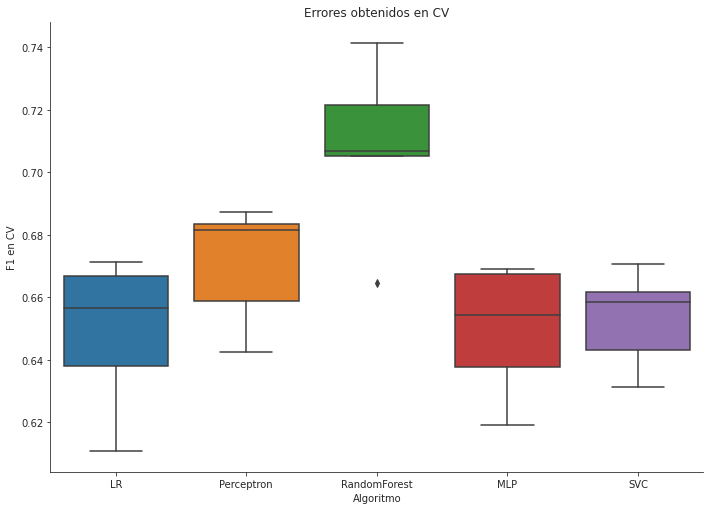
\includegraphics[width=1\textwidth]{images/box_plot}
    \caption{Puntuación F1 sobre los mismos conjuntos de validación cruzada}
\end{figure}

En este gráfico podemos ver que el algoritmo de regresión logistica consigue
resultados muy parecidos en todas las particiones que se han realizado. También
apreciamos como existen mejores resultados en general en los algoritmos de
random forest y perceptron pero hay un conjunto de validación para el que los
rendimientos son muy pobres y lastran el resultado final de la media.

Por el razonamiento que ya se ha expuesto sobre el problema que supone el
desbalanceo en las dos clases, creemos que no es suficiente utilizar la métrica 
$F1$ para decantarnos por un modelo u otro. 

El estudio de la curva ROC como se menciona en \cite{curves} no es muy
interesante ya que las clases presentan un desbalanceo moderado entre ellas y
por tanto nos hemos decantado por realizar un estudio de la curva
\textit{precission-recall}. Este tipo de curva representa en el eje vertical el
valor predicho para la clase positiva y en el eje horizontal el verdadero ratio
de positivos. Para los modelos the regresión logistica, random forest y MLP que
son los que sklearn nos permite dibujar este tipo de gráficas hemos obtenido 
los siguientes resultados:

\begin{figure}[H]\centering
    \subfloat[Curva P-R para regresión logística]{\label{a}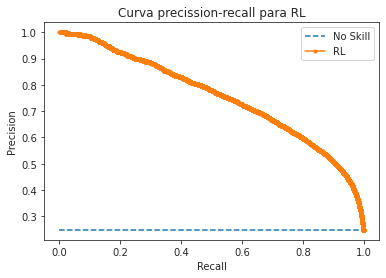
\includegraphics[width=.45\linewidth]{images/prlr}}\hfill
    \subfloat[Curva P-R para random forest]{\label{b}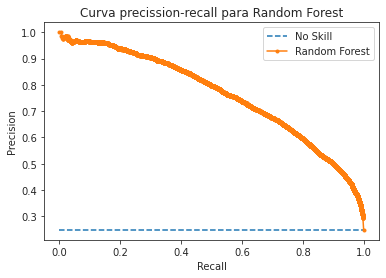
\includegraphics[width=.45\linewidth]{images/prrf}}\par 
    \subfloat[Curva P-R para MLP]{\label{c}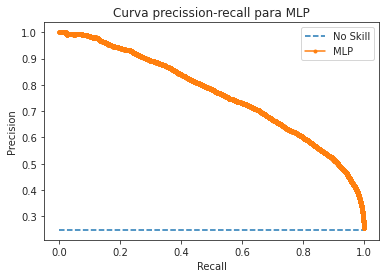
\includegraphics[width=.45\linewidth]{images/prmlp}}
    \caption{Curvas precission vs recall}
\end{figure}

Estas curvas no muestran un comportamiento óptimo, que sería una linea
horizontal en 1 que desciende al final pero si muestran un comportamiento 
que podemos considerar bueno. 

También creemos que es importante para comparar los modelos presentar la 
\textit{tabla de confusión} de los mismos. En esta tabla recogemos 

\begin{table}[H]
    \centering
    \begin{tabular}{lll}
                          &          Clase $\leq$ 50K        &       Clase $>$50K                \\ \cline{2-3} 
    \multicolumn{1}{l|}{Clase $\leq$ 50K} & \multicolumn{1}{l|}{verdadero positivo} & \multicolumn{1}{l|}{falso positivo} \\ \cline{2-3} 
    \multicolumn{1}{l|}{Clase $>$50K } & \multicolumn{1}{l|}{falso negativo} & \multicolumn{1}{l|}{verdadero negativo} \\ \cline{2-3} 
    \end{tabular}
    \caption{Significado de la matriz de confusión}
\end{table}

En el caso de los modelos estudiados dichas tablas son las siguientes

\textbf{Regresión logística}
\begin{table}[H]
\centering
\begin{tabular}{lll}
                          &          Clase $\leq$ 50K        &       Clase $>$50K                \\ \cline{2-3} 
\multicolumn{1}{l|}{Clase $\leq$ 50K} & \multicolumn{1}{l|}{25410} & \multicolumn{1}{l|}{2287} \\ \cline{2-3} 
\multicolumn{1}{l|}{Clase $>$50K } & \multicolumn{1}{l|}{3459} & \multicolumn{1}{l|}{5679} \\ \cline{2-3} 
\end{tabular}
\caption{Confusion matrix para regresión logística}
\end{table}

\textbf{Perceptrón}
\begin{table}[H]
\centering
\begin{tabular}{lll}
                          &          Clase $\leq$ 50K        &       Clase $>$50K                \\ \cline{2-3} 
\multicolumn{1}{l|}{Clase $\leq$ 50K} & \multicolumn{1}{l|}{24520} & \multicolumn{1}{l|}{3177} \\ \cline{2-3} 
\multicolumn{1}{l|}{Clase $>$50K } & \multicolumn{1}{l|}{3805} & \multicolumn{1}{l|}{5333} \\ \cline{2-3} 
\end{tabular}
\caption{Confusion matrix para Perceptrón}
\end{table}

\textbf{Random Forest}
\begin{table}[H]
\centering
\begin{tabular}{lll}
                          &          Clase $\leq$ 50K        &       Clase $>$50K                \\ \cline{2-3} 
\multicolumn{1}{l|}{Clase $\leq$ 50K} & \multicolumn{1}{l|}{25537} & \multicolumn{1}{l|}{2160} \\ \cline{2-3} 
\multicolumn{1}{l|}{Clase $>$50K } & \multicolumn{1}{l|}{3475} & \multicolumn{1}{l|}{5663} \\ \cline{2-3} 
\end{tabular}
\caption{Confusion matrix para Random Forest}
\end{table}

\textbf{Perceptrón Multicapa}
\begin{table}[H]
\centering
\begin{tabular}{lll}
                          &          Clase $\leq$ 50K        &       Clase $>$50K                \\ \cline{2-3} 
\multicolumn{1}{l|}{Clase $\leq$ 50K} & \multicolumn{1}{l|}{25530} & \multicolumn{1}{l|}{2167} \\ \cline{2-3} 
\multicolumn{1}{l|}{Clase $>$50K } & \multicolumn{1}{l|}{3493} & \multicolumn{1}{l|}{5645} \\ \cline{2-3} 
\end{tabular}
\caption{Confusion matrix para Perceptrón Multicapa}
\end{table}

\textbf{SVC}
\begin{table}[H]
\centering
\begin{tabular}{lll}
                          &          Clase $\leq$ 50K        &       Clase $>$50K                \\ \cline{2-3} 
\multicolumn{1}{l|}{Clase $\leq$ 50K} & \multicolumn{1}{l|}{25443} & \multicolumn{1}{l|}{2254} \\ \cline{2-3} 
\multicolumn{1}{l|}{Clase $>$50K } & \multicolumn{1}{l|}{3752} & \multicolumn{1}{l|}{5386} \\ \cline{2-3} 
\end{tabular}
\caption{Confusion matrix para SVC}
\end{table}

En estas tablas se puede comprobar como la semejanza que existía en la
puntuación que arrojaba la métrica $F1$, se ha traducido en unos valores casi
idénticos en las distintas entradas de las matrices de confusión. Esto nos dice
que en principio no existe un motivo para elegir un modelo sobre otro en función
de la clase que queramos predecir con mayor rigor. 

Por último para decantarnos por un modelo u otro hemos decidido evaluarlos con
la métrica accuracy y obtener un error de test con el que poder comparar los
resultados que obtenemos con cada modelo.

\begin{table}[H]
    \centering
    \begin{tabular}{c|c|c|c|c|c|}
    \cline{2-6}
                           & RL & Perceptrón & Random Forest & MLP & SVC \\ \hline
    \multicolumn{1}{|l|}{$E_{test}$}  & 0.1631 & 0.156 & 0.1895  & 0.153  & 0.1537  \\ \hline
    \end{tabular}
    \caption{$E_{test}$ obtenido para cada modelo usando accuracy como métrica}
\end{table}

En función de los resultados obtenidos con las datos de los que disponemos el
mejor modelo que podemos elegir es \textit{Perceptrón multicapa} que es el que
ha obtenido menor error en el conjunto de test.

Sobre el error $E_{out}$ que esperamos de este modelo podemos decir que será
cercano al error $E_{test}$ que hemos obtenido en este experimento. No creemos
que sea adecuado ofrecer una cota más general ya que las que hemos visto son muy
laxas y son cotas teóricas más que prácticas. Por como se ha conducido el
experimento y por los resultados que se obtienen podemos decir que la cota del 
error $E_{out}$ será próxima en general al $E_{test}$ obtenido para este modelo
en esta sección.

\section{Conclusiones}

En este proyecto hemos tenido la oportunidad de estudiar un problema de
clasificación binaria en el que se nos presentaba el reto de trabajar con 
dos clases de datos de las que no teníamos igual número de muestras. 

Hemos aprendido técnicas que nos han permitido decantarnos por unos modelos y
entrenarlos con un criterio que creemos correcto y finalmente hemos estudiado
los resultados que se han obtenido discutiendo la ideonidad de elegir unos
frente a otros. 

Además creemos que ha sido especialmente interesante la igualdad que se ha
demostrado entre casi todos los modelos y como el modelo de Perceptrón,
pese a ser un modelo lineal, obtiene resultados próximos a otros modelos más
complejos a nivel teórico.


%comparación entre modelos lineales y no lineales
%los resultados 
%las gráficas 
%confusion matrix
%ideonidad de los modelos


%cosas que no se rellenar: porque gamma=scale, porque hemos decidido usar MLP y SVC
%revisar métrica
%\bibliographystyle{plain}
\bibliographystyle{plain}
\bibliography{refs}

\end{document}
